%!TEX root = Funktionalanalysis - Vorlesung.tex

\chapter{Metrische R{\"a}ume}

\begin{definition}
	\begin{enumerate}[label=\alph*\upshape)]
		\item Sei $M$ eine nichtleere Menge. Eine Abbildung $d: M \times M \rightarrow 	\MdR$ hei{\ss}t \begriff{Metrik} auf $M$, falls $\forall x, y, z \in M:$
			\begin{description}
				\item[$\hspace{0.5cm} (M1) \hspace{0.1cm} $] $d(x, y) \geq 0, \hspace{0.25cm} d(x, y) = 0 \gdw x = y $  (positive Definitheit)
				\item[$\hspace{0.5cm} (M2) \hspace{0.1cm} $] $d(x, y) = d(y, x)$  (Symmetrie)
				\item[$\hspace{0.5cm} (M3) \hspace{0.1cm} $] $d(x, z) \leq d(x, y) + d(y, z)$  (Dreiecksungleichung)
			\end{description}
			Das Tupel $(M, d)$ nennen wir dann einen metrischen Raum. 
		\item Eine Folge $(x_{n})_{n \geq 1} \subset M$ konvergiert gegen $x \in M$, falls
			\[ d(x_{n}, x) \rightarrow 0 \hspace{0.5cm} \text{für } n \rightarrow \infty \]	 
			Notation: $x = \lim_{n \rightarrow \infty} x_{n}$ (in $M$)
	\end{enumerate}
\end{definition}

\begin{bemerkung*}
Der Grenzwert einer konvergenten Folge ist stets eindeutig, denn: \\
Sei $(x_{n})_{n \geq  1} \subset M$ mit $\lim_{n \rightarrow \infty} x_{n} = x \in M$ und $\lim_{n \rightarrow \infty} x_{n} = y \in M$, dann folgt: 
	\begin{align*}
		d(x, y) & \leq d(x, x_{n}) + d(x_{n}, y) \\
				& \rightarrow 0 \text{ für } n \rightarrow \infty
	\end{align*}
	d.h. $d(x, y) = 0 \Rightarrow x = y$
\end{bemerkung*}

\begin{beispiel}
	\begin{enumerate}[label=\alph*\upshape)]
		\item Sei $X$ ein normierter Vektorraum und $M \subset X$ (nichtleere) Teilmenge. \\
		Dann definiert $d(x, y) := \| x - y\|, \hspace{0.25cm} x, y \in M$ eine Metrik auf $M$ \\
		Ein Unterschied hier: Eine Norm setzt eine lineare Struktur auf $X$ voraus, eine Metrik macht auch Sinn auf nicht-linearen Teilmengen.
		\item \label{bsp:1-diskreteMetrik} Sei $M$ eine nichtleere Menge, dann definieren wir die \begriff{diskrete Metrik} auf $M$ durch
			\[ d(x, y) := \begin{cases}1 &, x \neq y \\ 0 &, x = y\end{cases} \]
			Dann ist $(M, d)$ ein metrischer Raum und es gilt: 
				\[ x_{n} \rightarrow x \text{ in } M \gdw \exists N \in \MdN \text{ mit } x_{n} = x \hspace{0.25cm} \forall n \geq N \]
	\end{enumerate}	
\end{beispiel}

\begin{beispiel}  \label{bsp:1-4.3}
	\begin{enumerate}[label=\alph*\upshape)]	
		\item Sei $X$ ein Vektorraum und $p_{j}$ für $j \in \MdN$ Halbnormen auf $X$ mit der Eigenschaft, dass für jedes $x \in X \setminus \{ 0 \}$ ein $K \in \MdN$ exisitert mit $p_{K} > 0$. Dann definiert
			\[ d(x, y) := \sum_{j \geq 1} 2^{-j} \frac{p_{j}(x - y)}{1 + p_{j}(x -y)}, \hspace{0.5cm} x, y \in X \]
			eine Metrik auf $X$ mit
			\[ d(x_{n}, x) \rightarrow 0 \gdw p_{j}(x_{n} - x) \rightarrow 0 \hspace{0.25cm} (n \rightarrow  \infty) \hspace{0.25cm} \forall j \in \MdN \]
			Beweis siehe Übung
		\item Für $X = \MdK^{\MdN} = \{ (x_{n})_{n \geq 1}: x_{n} \in \MdK \}$ und $p_{j}(x) := |x_{j}|, j \in \MdN$ definiert also
			\[ d(x, y) = \sum_{j = 1}^{\infty} 2^{-j} \frac{|x_{j} - y_{j}|}{1 + |x_{j} - y_{j}|} \text{ gerade die komponentenweise Konvergenz auf } X \]
		\item In $\ell^{\infty}$ entspricht die Konvergenz bezüglich $\| \cdot \|_{\ell^{\infty}}$ gerade der gleichmä{\ss}igen Konvergenz der Folge $x_{n} := (x_{n, i})_{(i \in \MdN)}$ gegen $x := (x_{i})_{(i \in \MdN)}$
			\[ \| x_{n} - x \|_{\ell^{\infty}} = \sup_{i \in \MdN} | x_{n, i} - x_{i} | \rightarrow 0 \hspace{0.5cm} (n \rightarrow \infty) \]
		\item In $C[a, b]$ entspricht die Konvergenz bezüglich $\| \cdot \|_{\infty}$ ebenfalls die gleichmä{\ss}ige Konvergenz von Funktionen
			\begin{align*}
				f_{n} \rightarrow f \text{ in } [a, b] & \gdw \| f_{n} - f \|_{\infty} = \sup_{t \in [a, b]} |f_{n}(t) - f(t) | \rightarrow 0 \\
				& \gdw f_{n} \rightarrow f \text{ gleichmä{\ss}ig.}
			\end{align*}
	\end{enumerate}
\end{beispiel}

\begin{definition} \label{def:1-4.4}
	Sei $(M, d)$ ein metrischer Raum.
	\begin{enumerate}[label=\alph*\upshape)]
		\item Eine Teilmenge $A \subset M$ hei{\ss}t \begriff{abgeschlossen} (in $M$), falls für alle in $M$ konvergenten Folgen $(x_{n})_{n \geq 1} \subset A$ der Grenzwert von $(x_{n})$ in $A$ liegt
		\item Eine Teilmenge $U \subset M$ hei{\ss}t \begriff{offen} (in $M$), falls zu jedem $x \in U$ ein $\epsilon > 0$ existiert, sodass
			\[ \{ y \in M: d(x, y) < \epsilon \} \subset U \]
	\end{enumerate}
\end{definition}

\begin{bemerkung} \label{bem:1-4.5}
	\begin{enumerate}[label=\alph*\upshape)] 
		\item Wir benutzen die Bezeichnungen
			\begin{align*}
				K(x, r) & := \{ y \in M: d(x, y) < r \} \hspace{0.25cm} \text{\textbf{ offene Kugel}} \\
				\bar K(x, r) & := \{ y \in M: d(x, y) \leq r \} \hspace{0.25cm}  \text{\textbf{ abgeschlossene Kugel}}
			\end{align*}
			für $x \in M, r > 0$. Man sieht leicht, dass $K(x, r)$ offen und $\bar K(x, r)$ abgeschlossen ist.
		\begin{beweis}
			\begin{enumerate}
			\item Sei $y \in K(x, r)$ und wähle $\rho := r - d(x, y) > 0$ \\
				Wir zeigen: $K(y, \rho) \subset K(x, r)$ (Dann ist $K(x, r)$ offen). Sei dazu $z \in K(y, \rho)$. Dann folgt 
				\begin{align*}
					d(x, y) \leq d(x, z) + d(z,y) & \leq r - \rho + d(z, y) \\
												  & \leq r - \rho + \rho = r \\ \\
								\Rightarrow z \in K(x, r)
				\end{align*} 
				Da $z$ beliebig war, folgt die Behauptung.
			\item Sei $(y_{n})_{n \geq 1} \subset \bar K(x, r)$ eine beliebige Folge mit $ \lim_{n \rightarrow \infty} y_{n} = y \in M$. Wir müssen zeigen, dass $y \in \bar K(x, r)$ (Dann ist $\bar K(x, r)$ abgeschlossen). \\
				\begin{align*}
					d(x, y) & \leq d(x, y_{n}) + d(y_{n}, y) \\
							& \leq r + d(y_{n}, y) \rightarrow r \\ \\
						& \Rightarrow d(x, y) \leq r, \text{ d.h. } y \in \bar K(x, r).
				\end{align*} 
			\end{enumerate}	
		\end{beweis} 
		\item $\emptyset, M$ sind sowohl offen, als auch abgeschlossen (in $M$)
		\item Bezüglich der diskreten Metrik $d$ aus \hyperref[bsp:1-diskreteMetrik]{Beispiel 4.2 b)} ist $\{x\} \subset M$ offen für jedes $x \in M$, da
			\[ K(x, r) = \{ x \} \subset \{ x \} \text{ für } r \in (0, 1] \]
	\end{enumerate}	
\end{bemerkung}

Wir fassen als Nächstes die grundlegenden Eigenschaften offener und abgeschlossener Mengen zusammen.

\begin{prop}
	Sei $(M, d)$ ein metrischer Raum und $I$ eine beliebige Indexmenge
	\begin{enumerate}[label=\alph*\upshape)]
		\item $A \subset M$ ist abgeschlossen in $M$ genau dann, wenn $U = M \setminus A$ offen ist
		\item Für eine beliebige Familie von abgeschlossenen Mengen $(A_{i})_{i \in I}$ sind 
			\[ A := \bigcap_{i \in I} A_{i} \hspace{0.5cm} \text{ und } \hspace{0.5cm} A_{i_{1}} \cup \dotsc \cup A_{i_{N}} \hspace{0.25cm} (i_{1}, \dotsc, i_{N} \in I) \]
			abgeschlossen in $M$.
		\item Für eine beliebige Familie offenere Mengen $(U_{i})_{i \in I}$ sind
			\[ U := \bigcup_{i \in I} U_{i} \hspace{0.5cm} \text{ und } \hspace{0.5cm} U_{i_{1}} \cap \dotsc \cap U_{i_{N}} \hspace{0.25cm} (i_{1}, \dotsc, i_{N} \in I) \] 
			offen in $M$.
	\end{enumerate}
	\begin{beweis}
		\begin{enumerate}[label=\alph*\upshape)]
			\item Sei $U$ nicht offen. Dann existiert ein $x_{0} \in U$ und  ein $x_{n} \in K(x_{0}, \frac{1}{n})$ mit $x_{n} \notin U$, d.h. $x_{n} \in U^{c} = A \forall n \in \MdN$. \\
				Da $d(x_{n}, x_{0}) \leq \frac{1}{n} \rightarrow 0$ und $x_{0} \notin A$, ist $A$ nicht abgeschlossen. \\ \\
				Sei umgekehrt $A$ nicht abgeschlossen. Dann existiert eine Folge $(x_{n})_{n \geq 1} \subset A$ mit $\lim_{n \rightarrow \infty} x_{n} = x \notin A$, d.h. $x \in U$. \\
				Für beliebige $\epsilon > 0$ existiert dann ein $N_{\epsilon} \in \MdN$ mit $d(x_{n}, x) < \epsilon$  $\forall n \geq N_{\epsilon}$ \\	
				$\Rightarrow (x_{n})_{n \geq N_{\epsilon}} \subset K(x, \epsilon) \cap A = K(x, \epsilon) \cap U^{c} \\
				\Rightarrow \forall \epsilon > 0 $ ist $ K(x, \epsilon) \not\subset U, $ d.h. $U$ ist nicht offen.
			\item folgt aus a) \& c), da
				\[ M \setminus \bigcap_{i \in I} A_{i} = \bigcup_{i \in I} M \setminus A_{i} \]
			\item Sei $x \in U$. Dann exisitert ein $U_{i_{0}}$ mit $x \in U_{i_{0}}$
			\[ \Rightarrow \exists r > 0: K(x, r) \subset U_{i_{0}} \subset U, \text{ d.h. } U \text{ ist offen.}  \]
			Sei $x \in U_{i_{1}} \cap \dotsc \cap U_{i_{N}}.$ Dann existieren $r_{1}, \dotsc, r_{N} > 0$ mit
			\[ K(x, r_{n}) \subset U_{i_{n}} \hspace{0.5cm} n = 1, \dotsc, N \]
			Setze $r := \min \{ r_{1}, \dotsc, r_{n} \} > 0$. Dann ist $K(x, r) \subset U_{i_{n}} \hspace{0.25cm} \forall n \in \{ 1, \dotsc, N \}$
			\[ \Rightarrow K(x, r) \subset U_{i_{1}} \cap \dotsc \cap U_{i_{N}}, \]
			d.h. $U_{i_{1}} \cap \dotsc \cap U_{i_{N}}$ ist offen.
		\end{enumerate}	
	\end{beweis}
\end{prop}

\begin{definition} \label{def:1-4.7-abschinnrand}
	Sei $(M, d)$ ein metrischer Raum und $V \subset M$. Dann hei{\ss}t 
	\begin{enumerate}[label=\alph*\upshape)]
		\item $\bar V := \bigcap \{ A \subset M: A$ ist abgeschlossen mit $V \subset A \} $ der \begriff{Abschluss} von $V$.
		\item $\mathring V := \bigcup \{ U \subset M: U$ ist offen mit $U \subset V \}$ das \begriff{Innere} von $V$. 
		\item $ \partial V := \bar V \setminus \mathring V$ der \begriff{Rand} von $V$.
	\end{enumerate}
\end{definition}

Hierfür gelten die folgenden Eigenschaften:

\begin{prop} \label{prop:1-4.8}
	Sei $(M, d)$ ein metrischer Raum und $V \subset M$
	\begin{enumerate}[label=\alph*\upshape)]
		\item
			\begin{enumerate}
				\item \label{prop:1-4.8.a1} $\bar V$ ist die kleinste abgeschlossene Menge, die $V$ enthält.
				\item \label{prop:1-4.8.a2} $V$ ist abgeschlossen $\gdw V = \bar V$
				\item \label{prop:1-4.8.a3} $\bar V = \{ x \in M: \exists (x_{n}) \subset V$ mit $\lim_{n \rightarrow \infty} x_{n} = x \} =: \tilde V$
			\end{enumerate} 
		\item 
			\begin{enumerate}
				\item \label{prop:1-4.8.b1} $\mathring V$ ist die grö{\ss}te offene Teilmenge von $V$.
				\item \label{prop:1-4.8.b2} $V$ ist offen $\gdw V = \mathring V$
				\item \label{prop:1-4.8.b3} $\mathring V = \{ x \in M: \exists \epsilon > 0$ mit $K(x, \epsilon) \subset V \} =: \hat V$
			\end{enumerate} 
		\item
			\begin{enumerate}
				\item \label{prop:1-4.8.c1} $\partial V$ ist abgeschlossen.
				\item \label{prop:1-4.8.c2} $\partial V = \{ x \in M: \exists (x_{n}) \subset V, (y_{n}) \subset M \ V$ mit $ \lim_{n \rightarrow \infty} x_{n} = \lim_{n \rightarrow \infty} y_{n} = x \}$
			\end{enumerate} 
	\end{enumerate}	
	\begin{beweis}
		\begin{enumerate}[label=\alph*\upshape)]
			\item
				\begin{enumerate}
					\item \label{prop:1-4.8.a1-proof} Nach Definition gilt $V \subseteq \bar V$ und $\bar V$ ist nach \hyperref[prop:1-4.8]{Proposition 4.7} abgeschlossen. \\
						Falls $V \subseteq A \subseteq \bar V$ und $A$ abgeschlossen, dann gilt $\bar V \subseteq A$ nach der Definition von $\bar V$, d.h. $A = \bar V$.
					\item folgt aus \hyperref[prop:1-4.8.a1]{(i)}
					\item Per Definition ist $\tilde V$ abgeschlossen, denn zu $(x_{n}) \subseteq \tilde V$ mit $\lim_{n \rightarrow \infty} x_{n} = x \in M$ existieren Folgen $(x_{n, m})_{m \geq 1}$ mit  $\lim_{m \rightarrow \infty} x_{n, m} = x_{n}$. \\
						Dann folgt aber für $(x_{n, n})_{n \geq 1} \subseteq V$:
						\[ d(x, x_{n, n}) \leq d(x, x_{n}) + d(x_{n}, x_{n, n}) \rightarrow 0 \text{ für } n \rightarrow \infty \]
						d.h. $x \in \tilde V$. Sei nun $A \subseteq M$ abgeschlossen mit $V \subseteq A$. Dann gilt nach \hyperref[def:1-4.4-abgoff]{Definition 4.4} $\tilde V \subseteq A$ und nach \hyperref[prop:1-4.8.a1]{(i)} damit $\bar V = \tilde V$.
				\end{enumerate} 
			\item 
				\begin{enumerate}
					\item zeigt man wie \hyperref[prop:1-4.8.a1-proof]{a) (i)}
					\item folgt aus \hyperref[prop:1-4.8.b1]{(i)}
					\item $\hat V$ ist per Definition offen, denn zu $x \in \hat V$ existiert ein $\epsilon > 0$ mit  $K(x, \epsilon) \subseteq V$. \\
						 Dann existiert aber zu jedem $y \in K(x, \epsilon)$ ein $\delta > 0$ mit $K(y, \delta) \subseteq K(x, \epsilon) \subseteq V$, d.h. $y \in \hat V$. $\Rightarrow K(x, \epsilon) \subseteq \hat V$ \\
						 Falls nun $U \subseteq V$ offen, so ist nach \hyperref[def:1-4.4-abgoff]{Definition 4.4} $U \subset \hat V$ und somit $\mathring V = \hat V$ nach \hyperref[prop:1-4.8.b1]{(i)}
				\end{enumerate} 
			\item
				\begin{enumerate}
					\item Da $\partial V = \overline{V} \cap (\mathring{V})^{c}$ ist $\partial V$ als Schnitz zweier abgeschlossenen Mengen wieder abgeschlossen.
					\item Nach \hyperref[def:1-4.7-abschinnrand]{Definition 4.6} gilt $(\mathring{V})^{c} = \overline{V^{c}}$ \quad (und $\left( \bar V \right)^{c} = \left( V^{c} \right)^{\circ}$) \\
						Damit folgt die Behauptung auf $\partial V = \bar V_{n} \cap \bar V^{c}$ und \hyperref[prop:1-4.8.a1]{a)}
				\end{enumerate} 
		\end{enumerate}	
	\end{beweis}
\end{prop}

\begin{definition} \label{def:1-4.9}
	Sei $(M, d)$ ein metrischer Raum
	\begin{enumerate}[label=\alph*\upshape)]
		\item Eine Menge $V \subset M$ hei{\ss}t \begriff{dicht} in M, falls $\bar V = M$, d.h. jeder Punkt in $M$ ist Grenzwert einer Folge aus $V$.
		\item $M$ hei{\ss}t \begriff{seperabel}, falls es eine abzählbare Teilmenge $V \subset M$ gibt, die dicht in $M$ liegt.
	\end{enumerate}
\end{definition}

\begin{bemerkung}
	\begin{enumerate}[label=\alph*\upshape)]
		\item All die Begriffe und Bezeichnungen aus \hyperref[def:1-4.4-abgoff]{Definition 4.4}, \hyperref[bem:1-4.5]{Bemerkung 4.5}, \hyperref[def:1-4.7-abschinnrand]{Definition 4.7} und \hyperref[def:1-4.9]{Definition 4.9} werden wir auch in normieren Räumen benutzen bzgl. der kanonischen Metrik $d(x, y) = \| x - y\|$
		\item Sei $(M, d)$ ein metrischer Rauam, $U \subset M$. Dann ist auch $(U, d)$ ein metrischer Raum. Für $V \subset U$ muss man dann aber unterscheiden bzgl. Abgeschlossenheit (bzw. Offenheit) von $V$ in $U$ oder in $M$. Man sagt dann, dass $V$ \begriff{relativ offen} bzw. \begriff{relativ abeschlossen} in $U$ ist.
	\end{enumerate}	
\end{bemerkung}

\begin{beispiel} \label{bsp:1-4.11}
	\begin{enumerate}[label=\alph*\upshape)]
		\item \label{bsp:1-4.11.a} Sei $X$ ein normierter Vektorraum (!), $x \in X, r > 0$. Dann gilt
			\begin{enumerate}
				\item $\bar K(x, r) = \overline{K(x, r)}$ \label{bsp:1-4.11.a.i}
				\item $\bar K(x, r)^{\circ} = K(x, r)$ \label{bsp:1-4.11.a.ii}
				\item $\partial \bar K(x, r) = \partial K(x, r) (= \{ y \in X: \| x - y \| = r \} ) $	\label{bsp:1-4.11.a.iii}
			\end{enumerate}
			\begin{beweis}
				\begin{enumerate}
					\item Da $ \bar K(x, r)$ abgeschlossen ist mit $K(x, r) \subset \bar K(x, r)$ folgt aus \hyperref[prop:1-4.8.a1]{Proposition 4.8  a) (i)} $\overline{K(x, r)} \subset \bar K(x, r)$.
						Sei umgekehrt $y \in \bar K(x, r)$ und $y_{n} = y - \frac{1}{n} (y - x), n \in \MdN$. Dann ist $y_{n} \in K(x, r)$ mit $\lim_{n \rightarrow \infty} y_{n} = y$, d.h. $y \in \overline{K(x, r)}$ nach \hyperref[prop:1-4.8.a3]{Proposition 4.8 a) (iii)}.
					\item Da $K(x, r)$ offen ist mit $K(x, r) \subset \bar K(x, r)$ folgt mit \hyperref[prop:1-4.8.b2]{Proposition 4.8 b) (ii)}: 
						\[ K(x, r) \subset \bar K(x, r)^{\circ} \]
						Sei umgekehrt $y \in \bar K(x, r)^{\circ}$. Dann existiert ein $\epsilon > 0$ mit $K(y, \epsilon) \subseteq \bar K(x, r)$. \\
						Angenommen $\| x - y \| = r$. Setze in diesem Fall $z := y + \frac{\epsilon}{2 r} (y - x)$. Dann gilt $z \in K(y, \epsilon)$, aber $z \notin \bar K(x, r)$, was zu einem Widerspruch führt. \\
						Also ist $\| x - y \| < r$, d.h. $y \in K(x, r)$.
					\item Aussage über Rand folgt aus \hyperref[bsp:1-4.11.a.i]{i)} und \hyperref[bsp:1-4.11.a.ii]{ii)}		
				\end{enumerate}
			\end{beweis}
		\item Die Aussagen in \hyperref[bsp:1-4.11.a]{a)} sind im Allgemeinen falsch für metrische Räume. \\
			Sei $M$ nichtleer mit mindestens 2 Elementen und $d$ die diskrete Metrik, dann gilt:
			\[ K(x, 1) = \{ x \}, \quad \bar K(x, 1) = M, \quad \overline{K(x, 1)} = \{ x \} \]
			$\Rightarrow \overline{K(x, 1)} \subsetneq \bar K(x, 1)$
		\item \label{bsp:1-4.11.b} Sei $X = C[0, 1]$ und $a, b > 0$ mit $a < b$. Dann ist die Menge
			\[ A := \{ f \in X: f(t) \in (a, b) \quad \forall t \in [0, 1] \} \]
			offen mit
			\begin{align*}
				\bar A & = \{ f \in X: f(t) \in [a, b] \quad \forall t \in [0, 1] \} \\
				\partial A & = \{ f \in \bar A: \exists t \in [0, 1] \text{ mit } f(t) \in \{ a, b \} \}
			\end{align*}
			\begin{beweis}
				\begin{enumerate} 
 					\item Sei $f \in A$ beliebig. \\ 		
						Da $f$ stetig auf $[0, 1]$ existieren $t_{1}, t_{2} \in [0, 1]$ mit
						\begin{align*}
							f(t_{1}) & = \min_{t \in [0, 1]} f(t) =: c_{1} > a \\
							f(t_{2}) & = \max_{t \in [0, 1]} f(t) =: c_{2} < b
						\end{align*}
						\begin{figure}[h]
  							\begin{center}
   								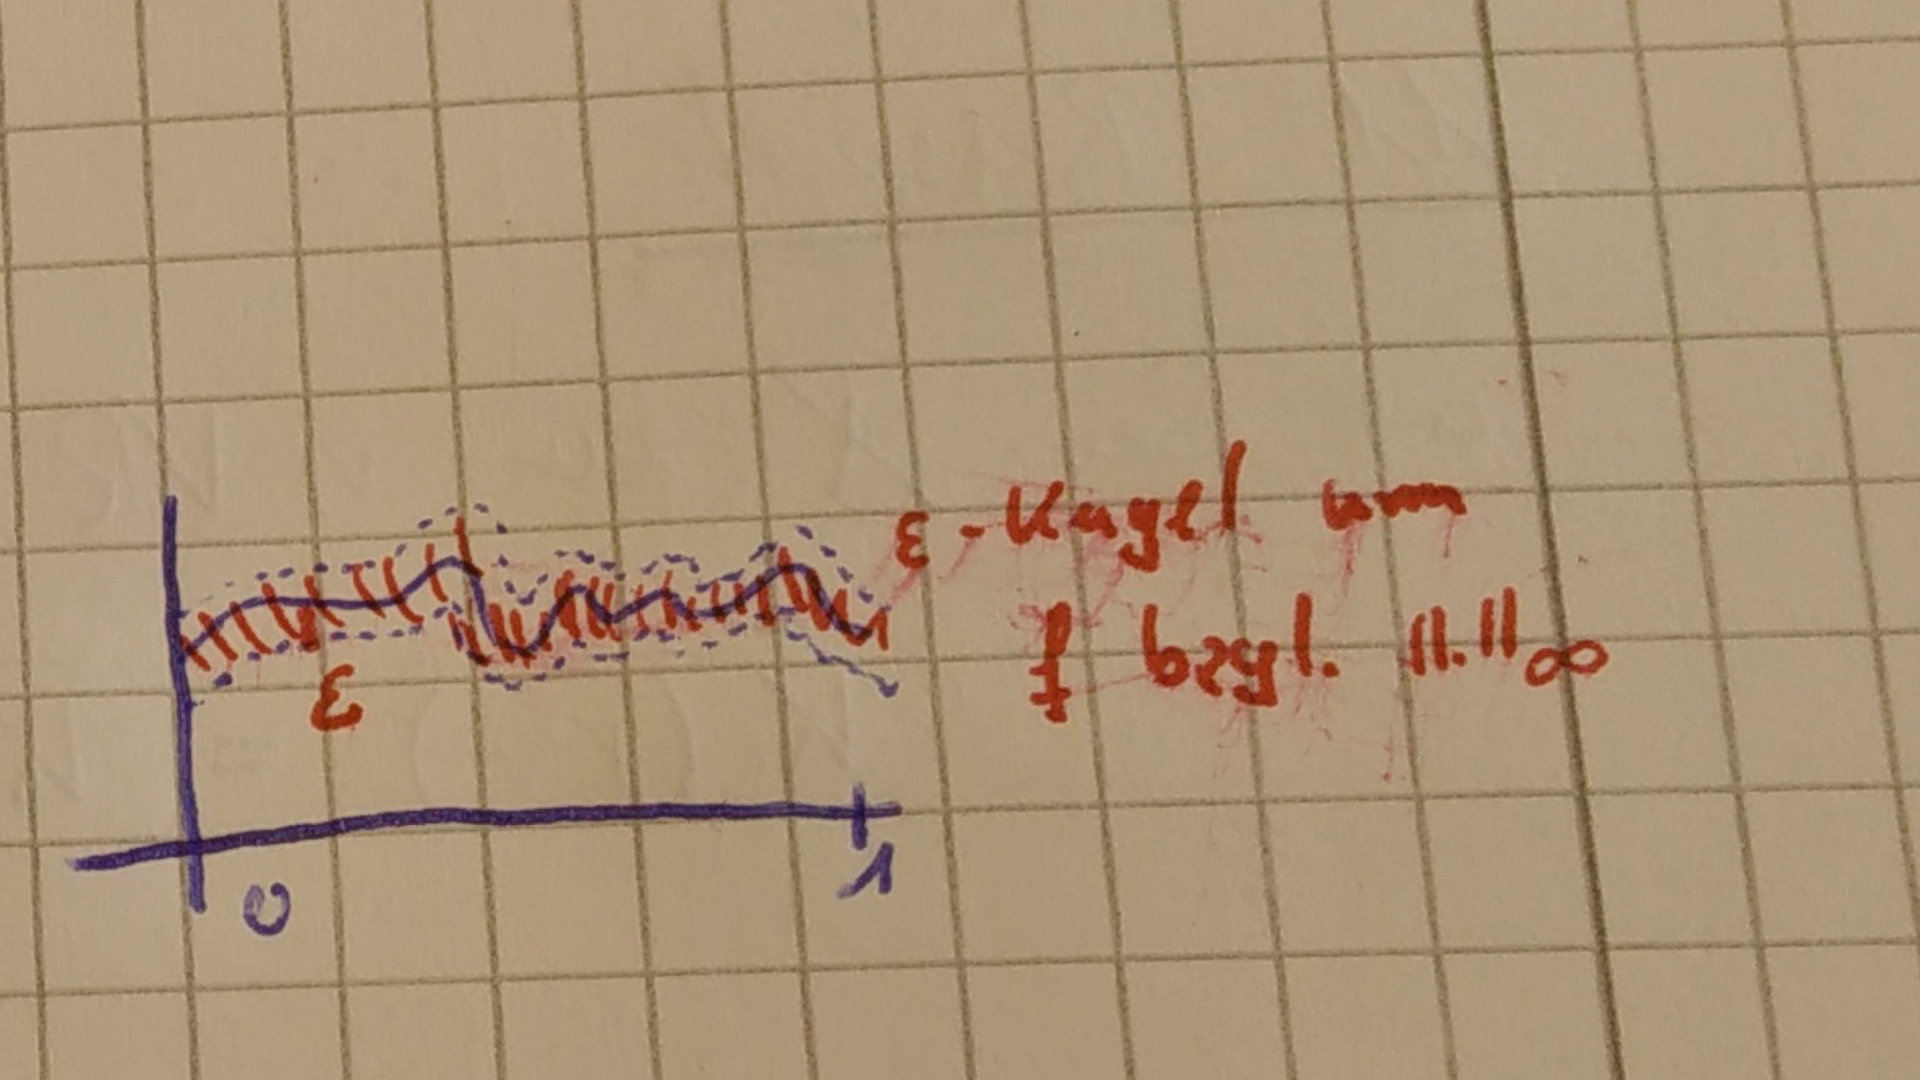
\includegraphics[width=0.48\textwidth]{images/bsp-4.11.c.i}					
  							\end{center}
						\end{figure}					
						Für $\epsilon \in (0, \min\{c_1 - a, b - c_2\})$ gilt dann $K(f, \epsilon) \subseteq A$, d.h. $A$ ist offen.
					\item Da Konvergenz bezüglich $\| \cdot \|_{\infty}$ punktweise Konvergenz impliziert, folgt direkt
						\[ \overline{A} \subseteq \{ f\in X \colon f(t) \in [a, b] \quad \forall t \in [a,b] \}. \]
						Ist umgekehrt $f \in X$ mit $f(t) \in [a, b]$ für alle $t \in [0,1]$, so definieren wir
						\[ f_{n}(t) = \begin{cases} a + \frac{1}{n} &, f(t) \leq a + \frac{1}{n} \\ b - \frac{1}{n} &, f(t) \geq b - \frac{1}{n} \\ f(t) &, \text{ sonst.}  \end{cases}   \]
						\begin{figure}[h]
  							\begin{center}
   								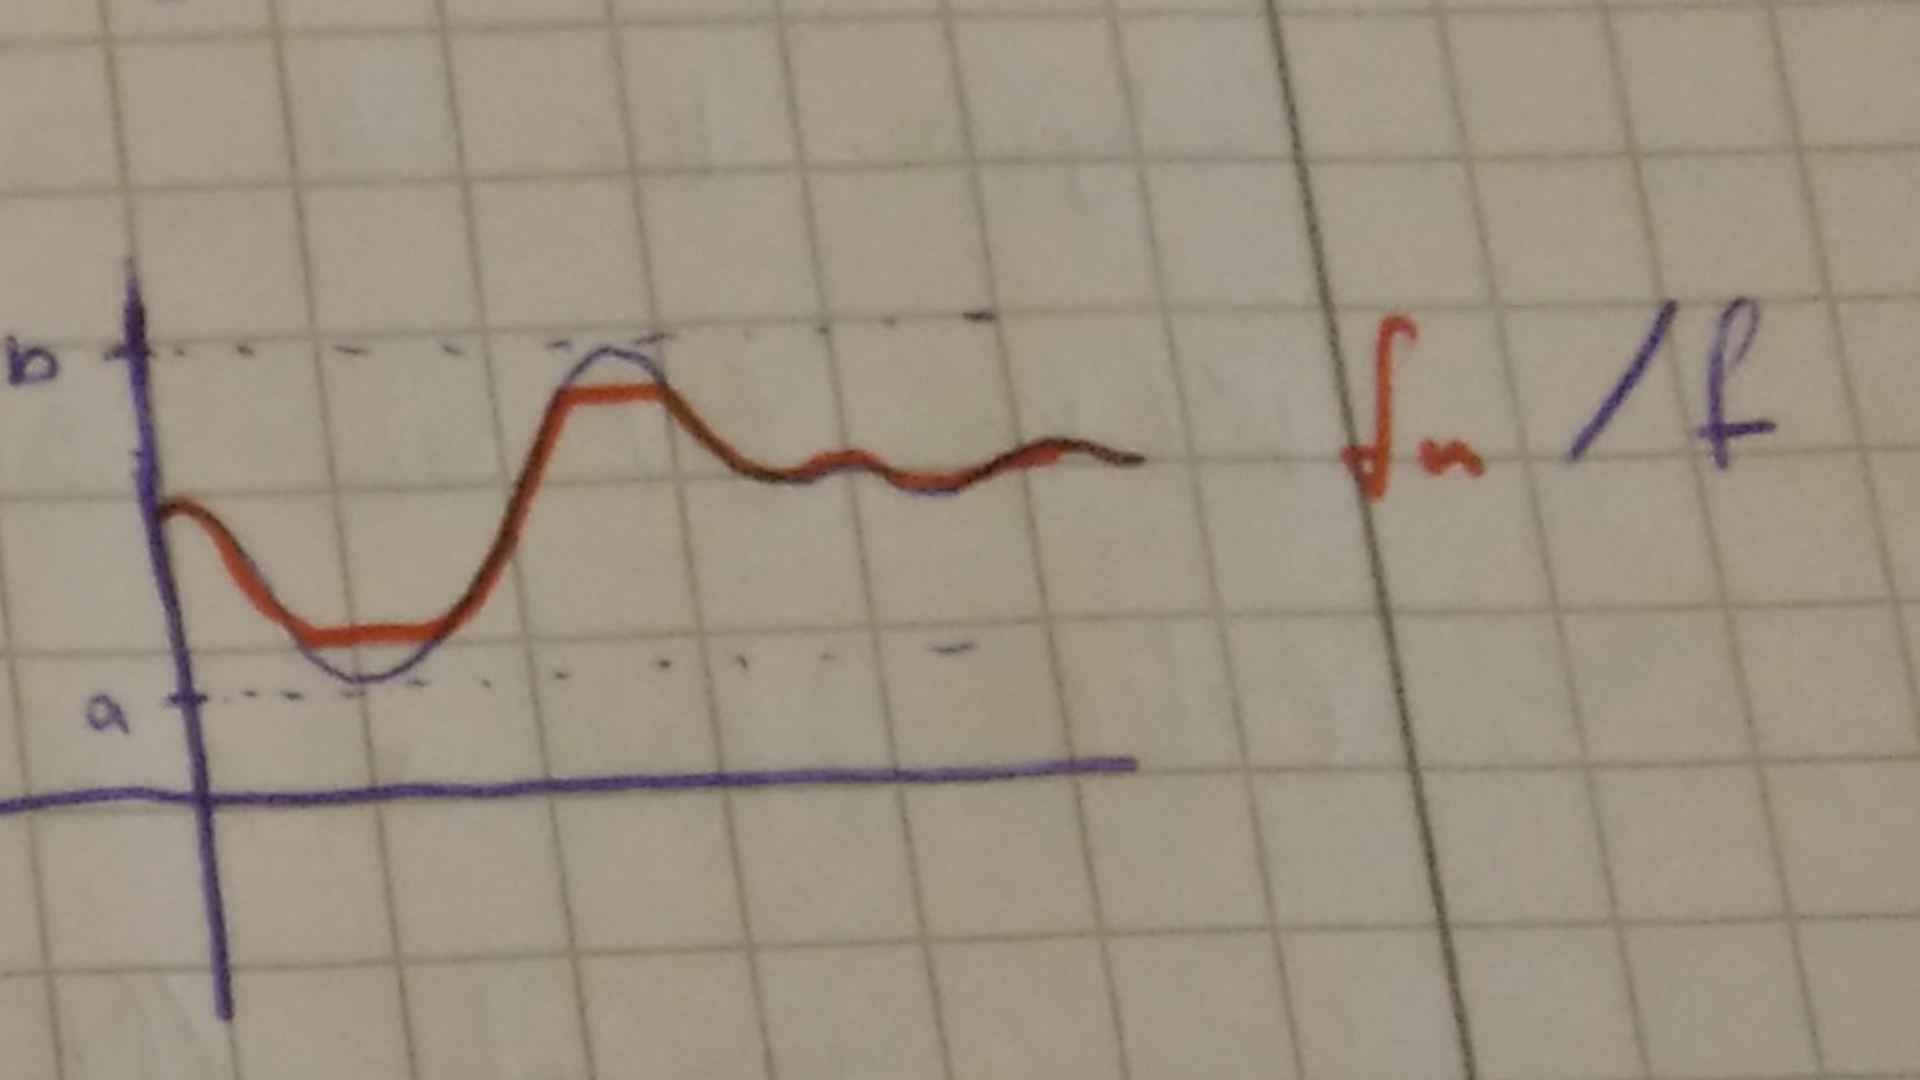
\includegraphics[width=0.48\textwidth]{images/bsp-4.11.c.ii}					
  							\end{center}
						\end{figure}		
						\[ \Rightarrow f_{n} \in A \text{ mit } \| f_{n} - f \|_{\infty} \rightarrow 0 \text{ } (n \rightarrow \infty) \text{, d.h. } f \in \bar A \]
					\item Aussage über $\partial A$ folgt aus \hyperref[bsp:1-4.11.b]{i)} und \hyperref[bsp:1-4.11.b]{ii)}
				\end{enumerate}
			\end{beweis}
		\item Sei $X$ ein normierter Vektorraum und $Y \subseteq X$ abzählbar mit $\overline{lin Y} = X$. Dann ist $X$ separabel.
			\begin{beweis}
				Wir definieren
				\[ lin_{\MdQ} Y := \{ y = \sum_{i = 1}^{n} q_{j} y_{j} : q_{j} \in \MdQ \quad (q_{j} \in \MdQ + i \MdQ ), y_{j} \in Y, n \in \MdN \} \]
				Dann ist $lin Y$ abzählbar, da $Y$ abzählbar ist. Sei nun $\epsilon > 0$ beliebig, $x \in X$. \\
				Nach Voraussetzung existiert dann ein $y \in lin Y$ mit $\| x - y \| < \epsilon$ \\
				Zu diesem $y$ finden wir ein $z \in lin_{\MdQ} Y$ mit $\| y - z \| < \epsilon$
				\[ \Rightarrow \| x - z \| < 2 \epsilon, \quad \text{d.h. } \overline{lin_{\MdQ} Y} = X \]
			\end{beweis}
		\item $C[0, 1]$ ist separabel, da $ lin \{ t^{n}, n \in \MdN \} $ dicht in $C[0, 1]$ liegt nach dem Approximationssatz von Weierstrass.
		\item Die Räume $\ell^{p}, p \in [1, \infty)$ und $c_{0}$ sind separabel, da
			\[ D = lin \{ e_{k}, k \in \MdK \} \text{ dicht in allen Räumen liegt.} \]
		\item Der Raum $\ell^{\infty}$ ist nicht separabel: \\
			Die Menge $\Omega$ der $\{0, 1\}$-wertigen Folgen ist überabzählbar. Für $x, y \in \Omega$ mit $x \neq y$ gilt $\| x - y \|_{\infty} = 1$ \\
			Angenommen: $\overline{ \{v_{k}, k \in \MdN \} } = \ell^{\infty}$. Dann
			\[ \Omega \subseteq \bigcup_{k \in \MdN} K \left( v_{k}, \frac{1}{4} \right) \]
			Wegen $\| x - y\|_{\ell^{\infty}} = 1$ $\forall x, y \in \Omega$ kann aber in jeder Kugel $K(v_{k}, \frac{1}{4})$ nur ein Element auf $\Omega$ liegen. 
			(d.h. zu $x \in \Omega$ existiert ein $k(x) \in \MdK$ mit $x \in K(v_{k(x)}, \frac{1}{4})$) \\
			$\Rightarrow$ die Abbildung $ J : \Omega \rightarrow \MdN, x \rightarrow k(x)$ ist injektiv \\
			$\Rightarrow \Omega$ ist abzählbar, Widerspruch.
	\end{enumerate}
\end{beispiel}

Schlie{\ss}lich betrachten wir Stetigkeit:

\begin{definition}
	Seien $(M, d_{M}), (N, d_{N})$ metrische Räume. \\
	Eine Abbildung $f: M \rightarrow N$ hei{\ss}t \textbf{stetig in $x_{0} \in M$}, falls für alle $(x_{n}) \subset M$ gilt
	\[ x_{n} \rightarrow x_{0} \text{ in } M \Rightarrow f(x_{n}) \rightarrow f(x_{0}) \text{ in } N \]
	\[ (d_{M}(x_{n}, x_{0}) \rightarrow 0 \hspace{0.25cm} (n \rightarrow \infty) \hspace{0.5cm} \Rightarrow \hspace{0.5cm} d_{N}(f(x_{n}), f(x_{0})) \rightarrow \hspace{0.25cm} (n \rightarrow \infty)) \]
	Die Abbildung $f$ hei{\ss}t \begriff{stetig} \textbf{auf $M$}, falls $f$ in jedem Punkt von $M$ stetig ist.
\end{definition}

Hierfür gelten folgende Eigenschaften:

\begin{prop} \label{prop:1-4.13}
	Sei $(K,d_{K}), (M, d_{M})$ und $(N, d_{N})$ metrische Räume und $f: M \rightarrow N, g: K \rightarrow M$. Dann gilt:
	\begin{enumerate}[label=\alph*\upshape)]
		\item Ist $g$ stetig in $x_{0}$, $f$ stetig in $g(x_{0})$, dann ist auch 
			\[ f \circ g: K \rightarrow N \text{ stetig in } x_{0} \]
		\item \label{prop:1-4.13.b} $f$ ist stetig in $x_{0} \in M$ genau dann, wenn 
			\[ \forall \epsilon > 0 \hspace{0.15cm} \exists \delta > 0 \hspace{0.15cm} \forall x \in M \text{ mit } d_{M}(x, x_{0}) < \delta \text{ gilt } d_{N}(f(x), f(x_{0})) < \epsilon \]
		\item Die folgenden Aussagen sind äquivalent:
			\begin{enumerate}
				\item $f$ ist stetig auf $M$
				\item Ist $U \subset N$ offen, so ist auch $f^{-1}(U)$ offen in $M$
				\item Ist $A \subset N$ abgeschlossen, so ist auch $f^{-1}(A)$ abgeschlossen in $M$.
			\end{enumerate}
	\end{enumerate}	
	\begin{beweis}		
		\begin{enumerate}[label=\alph*\upshape)]	
			\item Folgt direkt aus der Definition
			\item $" \Rightarrow "$: Annahme, das $\epsilon$-$\delta$-Kriterium gilt nicht. Dann existiert eine $\epsilon > 0$ und für jedes $n \in \MdN$ ein $x_{n} \in K(x_{0}, \frac{1}{n})$ mit $d_{M}(f(x_{n}), f(x_{0})) \geq \epsilon$. \\
				Dann gilt aber $d_{M}(x_{n}, x_{0}) < \frac{1}{n} \rightarrow 0$ für $n \rightarrow \infty$ und $d_{N}(f(x_{n}, f(x_{0})) \geq \epsilon \not\rightarrow 0$ für $n \rightarrow \infty$, d.h. $f$ ist nicht stetig in $x_{0}$. \\ \\
				$" \Leftarrow "$: Es gelte das $\epsilon$-$\delta$-Kriterium. Sei $(x_{n}) \subseteq M$ mit $x_{n} \rightarrow x_{0}, \epsilon > 0$. \\
				Dann gilt $d_{N}(f(x_{n}), f(x_{0})) < \epsilon$ für $n$ gro{\ss} genug. Da $\epsilon > 0$ beliebig, folgt $d_{N}(f(x_{n}), f(f_{0})) \rightarrow 0$ für $n \rightarrow \infty$.
			\item $(i) \Rightarrow (iii)$: Sei $A \subseteq N$ abgeschlossen und $(x_{n}) \subseteq f^{-1}(A)$ mit $x_{n} \rightarrow x$ in $M$ für $n \rightarrow \infty$. Dann gilt nach $(i)$ $f(x_{n}) \rightarrow f(x)$ in $N$ für $n \rightarrow \infty$. \\
				Da $(f(x_{n}))_{n \geq 1} \subseteq A$ und $A$ abgeschlossen ist, folgt $f(x) \in A$, d.h. $x \in f^{-1}(A)$. \\
				Also ist $f^{-1}(A)$ abgeschlossen. \\ \\
				$(iii) \Rightarrow (ii)$: Sei $U \subset N$ offen $\Rightarrow$ $U^{c}$ abgeschlossen $\Rightarrow$ $f^{-1}(U^{c}) = f^{-1}(U)^{c}$ ist abgeschlossen $\Rightarrow$ $f^{-1}(U)$ offen. \\ \\
				$(ii) \Rightarrow (i)$: 	Sei $x_{0} \in M$ beliebig. Für $\epsilon > 0$ ist nach $(ii)$ dann auch $f^{-1}(K(f(x_{0}), \epsilon))$ offen in M. \\
				Da $x_{0} \in f^{-1}(K(f(x_{0}), \epsilon))$, existiert ein $\delta > 0$ mit $K(x_{0}, \delta) \subseteq f^{-1}(K(f(x_{0}),\epsilon))$\\
				Das bedeutet gerade
				\[ \forall \epsilon > 0 \text{ } \exists \delta > 0: \forall x \in M \text{ mit } d_{M}(x_{0}, x) < \delta \text{ gilt auch} \]
				\[ d_{N}(f(x_{0}), f(x)) < \epsilon \]
				Nach \hyperref[prop:1-4.13.b]{b)} bedeutet dies gerade, dass $f$ stetig in $x_{0}$ ist.
		\end{enumerate}
	\end{beweis}
\end{prop}

\begin{beispiel}
	\begin{enumerate}[label=\alph*\upshape)]
		\item Sind $(M_{1}, d_{1}$ und $(M_{2}, d_{2})$ metrische Räume, so definiert
				\[ d(x, y) := d_{1}(x_{1}, y_{1}) + d_{2}(x_{2}, y_{2}) \]
			für $x = (x_{1}, x_{2}), y = (y_{1}, y_{2}) \in M_{1} \times M_{2}$ eine Metrik mit
			\[ d(x_{n}, x) \rightarrow 0 \gdw d_{1}(x_{n,1}, x_{1}) \rightarrow 0, d_{2}(x_{n,2}, x_{2}) \rightarrow 0 \]
			In diesem Sinne ist jede Metrik $d: M \times M \rightarrow \MdR$ stetig. Denn: \\
			Sei $(x_{n}, y_{n}) \rightarrow (x, y)$ in $M \times M$, d.h.
			\[ d(x_{n}, x) \rightarrow 0 \text{ und } d(y_{n}, y) \rightarrow 0 \hspace{0.5cm} (n \rightarrow \infty) \]
			\begin{align*}
				 d(x_{n}, y_{n}) - d(x, y) & \leq d(x_{n}, x) + d(x, y_{n}) - d(x, y) \\
										  & \leq d(x_{n}, x) + d(x, y) + d(y, y_{n}) - d(x, y) 		
			\end{align*}
			\[ d(x, y)- d(x_{n}, y_{n}) \leq \dotsc \leq d(x, x_{n}) + d(y_{n}, y) \]
			\[ \Rightarrow | d(x, y) - d(x_{n}, y_{n}) | \leq d(x, x_{n}) + d(y_{n}, y) \rightarrow 0 \hspace{0.5cm} (n \rightarrow \infty) \]
		\item Sei $X$ ein normierter Vektorraum und
			\begin{align*}
				A: \MdK \times X \rightarrow X, & \hspace{0.5cm} A( \alpha, x) = \alpha x \\
				S: X \times X \rightarrow X, & \hspace{0.5cm} S(x, y) = x + y
			\end{align*}
			Dann sind $A$ und $S$ stetig.
		\item Sei $X = C[0, 1], t_{0} \in [0, 1], \psi : X \rightarrow \MdK, \psi(f) = f(t_{0})$ \\
		Nach \hyperref[bsp:1-3.15]{Beispiel 3.15} ist $\psi$ stetig. D.h. ist $A \subset \MdK$ offen (abgeschlossen), so ist $\psi^{-1}(A)$ offen (abgeschlossen) nach \hyperref[prop:1-4.13]{Proposition 4.13}.
	\end{enumerate}	
\end{beispiel}

\newpage































